%!TEX program = xelatex

%\documentclass[UTF8]{ctexbeamer}
\documentclass[UTF8]{beamer}
\usetheme{Madrid}
%\usecolortheme{beaver}
\usepackage{graphicx}
\usepackage{amsmath}
\usepackage{amssymb}
\usepackage{float}
\usepackage{hyperref}
\usepackage{censor}
\usepackage{listings}
\usepackage{xcolor}
\usepackage{color}
\usepackage{textcomp}
\DeclareGraphicsExtensions{.eps,.ps,.jpg,.bmp,.png}



\definecolor{mygreen}{rgb}{0,0.6,0}
\definecolor{mygray}{rgb}{0.5,0.5,0.5}
\definecolor{mymauve}{rgb}{0.58,0,0.82}

\lstset{ %
%backgroundcolor=\color{white},      % choose the background color
basicstyle=\footnotesize\ttfamily,  % size of fonts used for the code
columns=fullflexible,
tabsize=4,
breaklines=true,               % automatic line breaking only at whitespace
captionpos=b,                  % sets the caption-position to bottom
commentstyle=\color{mygreen},  % comment style
escapeinside={\%*}{*)},        % if you want to add LaTeX within your code
keywordstyle=\color{blue},     % keyword style
stringstyle=\color{mymauve}\ttfamily,  % string literal style
frame=none,
rulesepcolor=\color{red!20!green!20!blue!20},
% identifierstyle=\color{red},
% language=c++,
}

%%Information to be included in the title page:
%\title{X}
%\author{Deli}
%%\institute{Deli institute}
%\date{\today}
%\title{Sequence alignment and search}
\title{Sequence alignment and search}

% [] {} 两个还是有区别的,具体的差异尝试编译一下就了解了。

%\subtitle{A review on alignment and search tools}
\subtitle{A review on alignment and search tools}
% 副标题,beamer的默认模板中基本上这些内容都有

\author[School of Life Science] % (optional, for multiple authors)
{Wenyuan Jiang\inst{1}}

\institute[Tongji University] % (optional)
{
	\inst{1}%
	School of Life Science\\
	Tongji University
}

\date[Mar 2021] % (optional)
{Class Presentation, Mar 2021}
%在每个section 前边单独插入当前章节高亮的目录页(当然最原始的目录页你还是需要手动录入的,不要想偷懒)
\AtBeginSection[]
{
	\begin{frame}
		\frametitle{Table of Contents}
		\tableofcontents[currentsection]
	\end{frame}
}

% 除了导言区所有内容都放到这里边来就对了
	    %	In this slide, some important text will be
	    %	\alert{highlighted} because it's important.
	    %	Please, don't abuse it.

\begin{document}
	\frame{\titlepage}
	\section{Background Information}

	\begin{frame}
	    \frametitle{How LARGE the data is}
		\begin{block}{Bit}<1->
			The bit is a basic unit of information in computing and digital communications. The bit represents a logical state with one of two possible values, 0 or 1.
		\end{block}
		\begin{block}{Byte}<2->
			The byte is a unit of digital information that most commonly consists of \alert{eight bits}. Usually, B represents byte and b represents bit.
		\end{block}
		\begin{block}{Magnitude}<3->
			B -> KiB -> MiB -> GiB -> TiB -> PiB -> EiB \dots

			(Each -> represents a magnitude of 1024.)
		\end{block}

    \end{frame}

	\begin{frame}
	    \frametitle{How FAST an algorithm is}
		\begin{block}{Big O notation}<1->
			Big O notation is a mathematical notation that describes the limiting behavior of a function when the argument tends towards a particular value or infinity.
		\end{block}
		\begin{block}{Formal definition}<2->
			Let $f$ be a real or complex valued function and g a real valued function. Let both functions be defined on some unbounded subset of the positive real numbers, and $g(x)$ be strictly positive for all large enough values of x.
			\begin{gather*}
				f(x)=O(g(x)) \space (x \rightarrow \infty)
			\end{gather*}
		\end{block}
    \end{frame}

	\begin{frame}
	    \frametitle{How FAST an algorithm is}
		\begin{block}{Application of Big O notation}<1->
			Big O notation can be used to compare the speed of different algorithm.
		\end{block}
		\begin{example}<2->
			Informally, especially in computer science, the big O notation often can be used to describe an asymptotic tight bound.
			For example, when considering a function $T(n) = 73n^3 + 22n^2 + 58$, we can say:
			\begin{gather*}
				T(n)=O(n^3)
			\end{gather*}
			Where $n$ often represents the data amount of an input, and $T(n)$ is the time for execution of an algorithm.
		\end{example}
    \end{frame}

	\begin{frame}
	    \frametitle{How FAST an algorithm is}
		\begin{block}{Comparing algorithms}<1->
			Big O notation can compare the absolute speed of an algorithm as well as the relative speed.
			\begin{itemize}
				\item $O(n log(n))$
				\item $O(n^k),(k>1)$
				\item $O(2^n)$
			\end{itemize}
		\end{block}
		\begin{example}<2->
			Bubble sort has a speed of $O(n^2)$, while Quick sort has a speed of $O(n log(n))$.

			Therefore, on the same machine (with the same amount of input $n$), Quick sort is faster than Bubble sort.
			If we run Quick sort on a slow machine and Bubble sort on a fast machine, when $n$ gets larger, Quick sort will \alert{eventually run faster} than Bubble sort.
		\end{example}
    \end{frame}

	\begin{frame}
	    \frametitle{How ACCURATE an algorithm is}
		\begin{block}{Traditional algorithms and Heuristic algorithms}<1->
			For Traditional algorithms, their output is definite and accurate.
			While for Heuristic algorithms, especially when ramdomness is involved, their output is not stable.
		\end{block}
		\begin{block}{Terminology}<2->
			\begin{itemize}
				\item TN, true negative
				\item FP, false positive
				\item FN, false negative
				\item TPR, true positive rate, $TPR = TP / P = TP / (TP+FN)$
				\item FPR, false positive rate, $FPR = FP / N = FP / (FP + TN)$
				\item ACC, accuracy, $ACC = (TP + TN) / (P + N)$
			\end{itemize}
		\end{block}
    \end{frame}

	\begin{frame}
	    \frametitle{How ACCURATE an algorithm is}
		\begin{block}{ROC curve}<1->
			The ROC curve is created by plotting the true positive rate (\alert{TPR}) against the false positive rate (\alert{FPR}) at various threshold settings.
		\end{block}
		\begin{figure}[H]
			\centering
			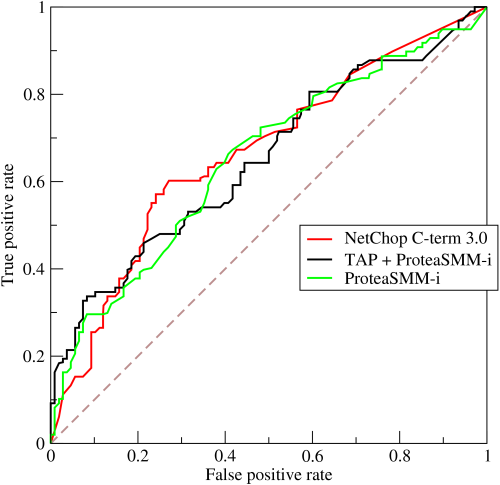
\includegraphics[width=0.4\textwidth]{image/Roccurves}
			\label{ROC-2}
		\end{figure}
    \end{frame}

	\begin{frame}
	    \frametitle{How ACCURATE an algorithm is}
		\begin{block}{AUC}<1->
			AUC is the area under the ROC curve.
		\end{block}
		\begin{example}
			\begin{figure}[H]
				\centering
				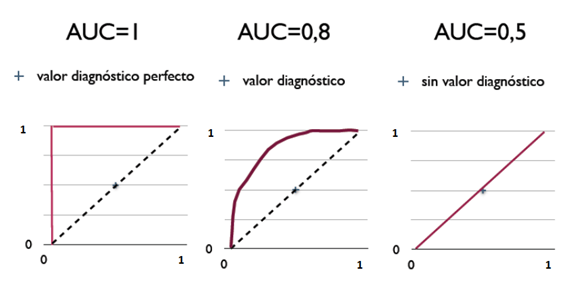
\includegraphics[width=0.7\textwidth]{image/Curvas}
				\label{ROC-3}
			\end{figure}
		\end{example}
    \end{frame}

    \section{Tools for sequence alignment and search}

	\begin{frame}
	    \frametitle{Pairwise alignment}
		\begin{block}{Pairwise alignment}<1->
			Pairwise sequence alignment methods are used to find the best-matching piecewise (local or global) alignments of \alert{two} query sequences. 
		\end{block}
		\begin{block}{Usage of Pairwise alignment}<2->
			Pairwise alignments can only be used between two sequences at a time, 
			but they are efficient to calculate and are often used for methods that do not require extreme precision 
			(such as searching a database for sequences with high similarity to a query).
		\end{block}
    \end{frame}

	\begin{frame}
	    \frametitle{Pairwise alignment}
		\begin{block}{Algorithms for Pairwise alignment}<1->
			\begin{itemize}
				\item Dot-matrix methods
				\item Dynamic programming
				\item Word methods
			\end{itemize} 
		\end{block}
    \end{frame}

	\begin{frame}
	    \frametitle{Pairwise alignment: Dot-matrix}
		\begin{block}{Dot-matrix methods}<1->
			The dot-matrix approach, which implicitly produces a family of alignments for individual sequence regions, 
			is qualitative and conceptually simple, though time-consuming to analyze on a large scale. 
			In the absence of noise, it can be easy to visually identify certain sequence features—such as insertions, deletions, repeats, or inverted repeats—from a dot-matrix plot. 
			To construct a dot-matrix plot, the two sequences are written along the top row and leftmost column of a two-dimensional matrix and a dot is placed at any point where the characters in the appropriate columns match—this is a typical recurrence plot.
		\end{block}
    \end{frame}

	\begin{frame}
	    \frametitle{Pairwise alignment}
		\begin{figure}[H]
			\centering
			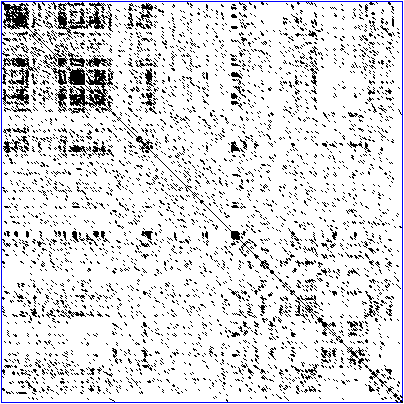
\includegraphics[width=0.5\textwidth]{image/Zinc-finger-dot-plot}
			\label{DOT-1}
		\end{figure}
	\end{frame}

	\begin{frame}
	    \frametitle{Pairwise alignment: Dot-matrix}
		\begin{block}{Dot-matrix tool}<1->
			\begin{itemize}
				\item Dotter: A dot-matrix program with interactive greyscale rendering for genomic DNA and Protein sequence analysis
			\end{itemize}
		\end{block}
		\begin{block}{Dot-matrix method advantage}<2->
			\begin{itemize}
				\item Fairly easy to Implement.
				\item Easy to understand visually.
				\item It shows all possible alignment of pairs.
				\item Good overview of places fot good alignment.
			\end{itemize}
		\end{block}
		\begin{block}{Dot-matrix method speed}<3->
			For two sequences that have the length of $n$:
			\begin{gather*}
				O(n^2)
			\end{gather*}
		\end{block}
    \end{frame}

	\begin{frame}
	    \frametitle{Pairwise alignment: Dynamic programming}
		\begin{block}{Dynamic programming}<1->
			The technique of dynamic programming can be applied to produce global alignments via the \alert{Needleman-Wunsch algorithm}, and local alignments via the \alert{Smith-Waterman algorithm}. 
			In typical usage, protein alignments use a \alert{substitution matrix} to assign scores to amino-acid matches or mismatches, 
			and a gap penalty for matching an amino acid in one sequence to a gap in the other. DNA and RNA alignments may use a scoring matrix, 
			but in practice often simply assign a positive match score, a negative mismatch score, and a negative gap penalty.
		\end{block}
    \end{frame}

	\begin{frame}
	    \frametitle{Pairwise alignment: Dynamic programming}
		\begin{block}{Input and output}<1->
			The input of the algorithm is two sequences, and the output is a score representing how similar the sequences are.
			On most cases, a pattern showing the matches will be given.

			For example:

			\texttt{TACGGGCCCGCTA-C}

			\texttt{||---|-||-|||-|}
			
			\texttt{TA---G-CC-CTATC}
		\end{block}
    \end{frame}

	\begin{frame}
	    \frametitle{Pairwise alignment: Dynamic programming}
		\begin{block}{Dynamic programming tool}<1->
			\begin{itemize}
				\item EMBOSS Water
				\item EMBOSS Needle
				\item \url{http://emboss.sourceforge.net/}
			\end{itemize}
		\end{block}
		\begin{block}{Dynamic programming method speed}<2->
			For two sequences that have the length of $n$:
			\begin{gather*}
				O(n^2)
			\end{gather*}
		\end{block}
    \end{frame}

	\begin{frame}
	    \frametitle{Pairwise alignment: Word methods}
		\begin{block}{Word methods}<1->
			Word methods, also known as k-tuple methods, are heuristic methods that are not guaranteed to find an optimal alignment solution, 
			but are significantly more efficient than dynamic programming. 
			These methods are especially useful in large-scale database searches where it is understood that a large proportion of the candidate sequences will have essentially no significant match with the query sequence.
		\end{block}
		\begin{block}{Word methods speed}<2->
			For two sequences that have the length of $n$:
			\begin{gather*}
				O(n^k),1<k<2
			\end{gather*}
		\end{block}
    \end{frame}

	\begin{frame}
	    \frametitle{Pairwise alignment: Word methods}
		\begin{block}{Word methods tool}<1->
			\begin{itemize}
				\item EMBL FASTA
				http://www.ebi.ac.uk/fasta33/
				\item NCBI BLAST
				https://blast.ncbi.nlm.nih.gov/Blast.cgi
			\end{itemize}
		\end{block}
    \end{frame}

	\begin{frame}
	    \frametitle{Multiple sequence alignment}
		\begin{block}{Modified pairwise alignment algorithms}<1->
			Most Pairwise alignment algorithms can be easily modified for Multiple sequence alignment. However, such algorithms are too slow to handle massive amount of data.
		\end{block}
		\begin{block}{Specialized agorithms and tools}<2->
			Some algorithms are designed for fast multiple sequence alignment, but most of them are not sensitive compared with Pairwise alignment algorithms.

			Below are some tools.
			\begin{itemize}
				\item Clustal
				\item T-Coffee
				\item LINCLUST
				\item \alert{MMseqs2}
				\item UCLUST
			\end{itemize}
		\end{block}
    \end{frame}

	\section{MMseqs2}

	\begin{frame}
	    \frametitle{MMseqs2 Publications}
		\begin{itemize}
			\item Steinegger M and Soeding J. MMseqs2 enables sensitive protein sequence searching for the analysis of massive data sets. Nature Biotechnology, doi: 10.1038/nbt.3988 (2017).
			\item Steinegger M and Soeding J. Clustering huge protein sequence sets in linear time. Nature Communications, doi: 10.1038/s41467-018-04964-5 (2018).
			\item Mirdita M, Steinegger M and Soeding J. MMseqs2 desktop and local web server app for fast, interactive sequence searches. Bioinformatics, doi: 10.1093/bioinformatics/bty1057 (2019).
			\item Mirdita M, Steinegger M, Breitwieser F, Soding J, Levy Karin E: Fast and sensitive taxonomic assignment to metagenomic contigs. bioRxiv, doi: 10.1101/2020.11.27.401018 (2020).
		\end{itemize}
    \end{frame}
	
	\begin{frame}[fragile]
		Before installation, \alert{read the documents of the source code carefully}, 
		and make sure you understand all the instructions in the doc.
	    \frametitle{Install MMseqs2}
		\begin{block}{Install gcc, cmake and libz}<1->
			To compile MMseqs2 \alert{\lstinline{git}, \lstinline{g++ (4.9 or higher)} and \lstinline{cmake (2.8.12 or higher)}} are needed.
			\lstinline{Zlib} and \lstinline{Bzlib} are optional.

			\lstinline{apt-get install build-essential cmake zlib1g zlib1g-devel libbz2-dev}
		\end{block}
		\begin{block}{Download source code}<2->
			\lstinline{git clone https://github.com/soedinglab/MMseqs2.git && cd MMseqs2}
		\end{block}
		\begin{block}{Compile and Install}<3->
			\lstinline{mkdir build && cd build/}

			\lstinline{cmake -DCMAKE_BUILD_TYPE=RELEASE -DCMAKE_INSTALL_PREFIX=/usr ..}

			\lstinline{make -j && make install}
		\end{block}

    \end{frame}

	\begin{frame}[fragile]
	    \frametitle{Use MMseqs2: Search}
		\begin{block}{Create a database}<1->
			You can create a database from a FASTA file.

			\lstinline{mmseqs createdb examples/DB.fasta targetDB}

			\lstinline{mmseqs createindex targetDB tmp}

			Or you can download a database online.

			\lstinline{mmseqs databases UniProtKB/Swiss-Prot swissprot tmp}
		\end{block}

		\begin{block}{Search}<2->
			You can search some sequences in a fasta file.

			\lstinline{mmseqs easy-search examples/QUERY.fasta examples/DB.fasta alnRes.m8 tmp}

			Or search some sequences in a pre-built database, which is much faster.

			\lstinline{mmseqs easy-search examples/QUERY.fasta targetDB alnRes.m8 tmp}

		\end{block}

    \end{frame}

	\begin{frame}[fragile]
	    \frametitle{Use MMseqs2: Search}

		\begin{block}{Search Results}<1->
			The results of a search is in \alert{m8 format}, which is a tab-separated ascii file with lines like this:

			\lstinline{A0A061HXN7 P13020 0.953 780 37 0 1 778 1 780 0.000E+00 1521}

			Each column has the definition listed below:
			\begin{itemize}
				\tiny
				\item Query id
				\item Subject id
				\item Identity
				\item Alignment length
				\item Mismatches
				\item Gap Openings
				\item q. start
				\item q. end
				\item s. start
				\item s. end
				\item e-value
				\item bit score
			\end{itemize}
		\end{block}

    \end{frame}

	\begin{frame}[fragile]
	    \frametitle{Use MMseqs2: Cluster}
		\begin{block}{Clustering FASTA files}<1->
			For clustering, MMseqs2 \lstinline{easy-cluster} and \lstinline{easy-linclust} are available.

			\lstinline{mmseqs easy-cluster examples/DB.fasta clusterRes tmp}

			\lstinline{mmseqs easy-linclust examples/DB.fasta clusterRes tmp}
		\end{block}

		\begin{block}{Cluster results}<2->
			The commands above produces three files: \lstinline{clusterRes_cluster.tsv}, 
			\lstinline{clusterRes_all_seqs.fasta} and \lstinline{clusterRes_rep_seq.fasta}.
		\end{block}

    \end{frame}

	\begin{frame}[fragile]
	    \frametitle{Use MMseqs2: Cluster}
		\begin{block}{Cluster results}<1->
			The \lstinline{clusterRes_cluster.tsv} file follows the following format:

			\begin{lstlisting}[frame=single]
#cluster-representative cluster-member
Q0KJ32                  Q0KJ32
Q0KJ32                  C0W539
Q0KJ32                  D6KVP9
...
\end{lstlisting}
		\end{block}

		\begin{block}{Cluster results}<2->
			The \lstinline{clusterRes_all_seqs.fasta} is FASTA-like format file, 
			with a new cluster being marked by two identical name lines of the representative sequence.

			The \lstinline{clusterRes_rep_seq.fasta} contains all representative sequences.
		\end{block}

    \end{frame}

	\begin{frame}[fragile]
	    \frametitle{MMseqs2: Performance}

		\begin{block}{Computing environment}<1->
			\begin{itemize}
				\item \lstinline{Hardware: Xeon Gold 5117 @2.00GHz 28C56T, 32GB RAM, SSD}
				\item \lstinline{Software: Ubuntu 18.04, MMseqs2 Release 13 compiled with gcc 7.5.0}
			\end{itemize}
		\end{block}

		\begin{block}{Data size}<2->
			The input file is \lstinline{swiss.fasta}, which contains \alert{\lstinline{1129276}} seqs from UniProtKB.
			The size of the file is \alert{\lstinline{264MB}}
		\end{block}
    \end{frame}

	\begin{frame}[fragile]
	    \frametitle{MMseqs2: Performance}

		\begin{block}{Performance}<1->
			Using command 
			
			\lstinline{time mmseqs easy-cluster examples/swiss.fasta clusterRes tmp} 
			
			to do the clustering, it took:
			\alert{\lstinline{1m21.693s}}.
		\end{block}

		\begin{block}{Performance}<2->
			Using command 
			
			\lstinline{time mmseqs easy-linclust examples/swiss.fasta clusterRes tmp} 
			
			to do the clustering, it took:
			\alert{\lstinline{0m16.869s}}.
		\end{block}
    \end{frame}

	\section{Possible future improvements}

	\begin{frame}
	    \frametitle{Algorithm?}
		\begin{itemize}
			\item Parallel computing?
			\item Machine learning based methods?
			\item Quantum computing?
		\end{itemize}
    \end{frame}

	\begin{frame}
	    \frametitle{Hardware?}
		\begin{itemize}
			\item GPU?
			\item CPU Clusters?
			\item FPGA?
			\item Playstation?
			\item \small Wirawan A, Kwoh C K, Hieu N T, et al. CBESW: sequence alignment on the playstation 3
		\end{itemize}
    \end{frame}

	\section{Q \& A}
	\begin{frame}
		\Huge{\centerline{Q \& A}}
	\end{frame}
	\begin{frame}
		\frametitle{References}
		\begin{itemize}
			\tiny
			\item Likic V. The Needleman-Wunsch algorithm for sequence alignment[J]. Lecture given at the 7th Melbourne Bioinformatics Course, Bi021 Molecular Science and Biotechnology Institute, University of Melbourne, 2008: 1-46.
			\item Nevill-Manning C G, Huang C N, Brutlag D L. Pairwise protein sequence alignment using Needleman-Wunsch and Smith-Waterman algorithms[J]. Personal communication (http://motif.stanford.edu/alion/), 1997.
			\item Higgins D G, Sharp P M. Fast and sensitive multiple sequence alignments on a microcomputer[J]. Bioinformatics, 1989, 5(2): 151-153.
			\item Steinegger M, Söding J. Clustering huge protein sequence sets in linear time[J]. Nature communications, 2018, 9(1): 1-8.
			\item Polyanovsky V O, Roytberg M A, Tumanyan V G. Comparative analysis of the quality of a global algorithm and a local algorithm for alignment of two sequences[J]. Algorithms for molecular biology, 2011, 6(1): 1-12.
			\item Wirawan A, Kwoh C K, Hieu N T, et al. CBESW: sequence alignment on the playstation 3[J]. BMC bioinformatics, 2008, 9(1): 1-10.
		\end{itemize}
	\end{frame}
\end{document}